\documentclass{projdoc}
\organization{Avans University of Applied Sciences}
\project{Project cr\^epe}
\author{%
	Loek Le Blansch\and%
	Wouter Boerenkamps\and%
	Jaro Rutjes\and%
	Max Smits\and%
	Niels Stunnebrink%
}


\title{Research document}

\begin{document}
\tablestables
\newpage

\section{Introduction}

\section{Game engine}

\subsection{Introduction}

To build a game engine, it must first be understood how it operates. The
functionalities it requires and how these functionalities work together must be
determined. In this section, the general functioning of a game engine and the
different parts required are described.

\subsection{Findings}

A game engine is not the game itself but a platform with which games are built. It
should provide the functionalities with which the game is constructed. The purpose of
a game engine is not to create data out of nothing. Instead, data is read, and the
correlating features and effects are generated. However, the engine is also used to
create these files, referred to as ``assets.'' The game engine must be able to accept
a certain format of these assets---whether levels, sprites, or textures---and convert
them into usable data.

\subsubsection{Layers}

A game engine is composed of multiple layers, each with its own functions. These
layers are divided into the following categories:\noparbreak
\begin{description}
	\item[Resource manager] Responsible for what happens when the engine is launched,
		including loading data formats.
	\item[Application] Manages the run loop, time, code execution, and events
		(e.g.~input events).
	\item[Window/\glspl{hid}] Handles input and events.
	\item[Renderer] Responsible for drawing the necessary objects on the screen,
		usually once per frame.
	\item[Debugging support] Provides testing for the engine, such as logging or
		performance profiling.
	\item[Scripting layer] Runs scripts, such as Lua or Python.
	\item[Memory systems] Handles and monitors memory usage.
	\item[Physics] Adds specific physics to objects.
	\item[Audio] Processes audio.
	\item[AI] Provides artificial inteligent behavior.
\end{description}

\subsubsection{Structure}

The above mentioned layers should be structured, somehow. One of the requirements is
that the game engine's API uses a so-called gameObject (with one or more component(s)).
The gameObject is described in more detail at \cref{sec:Gameobjects/components}.

There are multiple structures that could be used to structure a game engine. It's of
course possible to use inheritance. A major disadvantages of inheritance is that it's
not flexible. However, the provided class diagram of the game engine's API already
specifies that composition should be used (in stead of inheritance). So, let's take a
look at structures that use composition.

The Decorator design pattern (as shown in \cref{fig:decorator}) could be used to structure
the game engine. A gameObject's propperties/behavior is determined by one (or more)
components. The Decorator design pattern allows to modify an object's propperties/behavior
by adding one (or more) Decorators. The object that is modified, could be the gameObject and
the components could be the Decorators. This is not exactly the same as the required API,
but it's very close. A major disadvantage of such Decorator design pattern, is that the
interface of all components should be the same (they should share the same methods), because
the client (which is the scene in our case) can only call/reach the components through the
interface. This would require very general methods (at the interface), which might make the
programming harder. \autocite{man:DecoratorDesignPattern} \autocite{man:Decorator}
\begin{figure}[H]
    \centering
    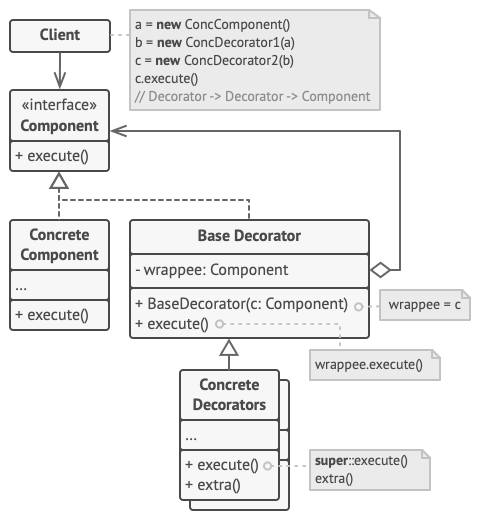
\includegraphics[width=0.5\textwidth]{img/DecoratorDesignPattern.png}
    \caption{Decorator design pattern \autocite{img:Decorator}}
    \label{fig:decorator}
\end{figure}

Another very popular design pattern, is the Entity Component System (\gls{ecs}). ...

\paragraph{ECS}

A game engine must have the ability to keep track and update several game objects. To
do this most game engines employ an \gls{ecs} model which uses modulair components to
give entities properties and features. The need for an entity component system arises
because multiple game objects are required to create a scene in a game. These game
objects exist within the scene and perform actions, such as a UI display for a score.
This game object does not need to be rendered; it could be a script running in the
background. It could also be a player sprite that is controlled. These entities need
to be aware of other entities, for example, during collisions. For this to function,
a scene is required to host all game objects. Within this scene, the game objects
must be stored efficiently, and entities must be provided with the required behavior,
such as audio, position, or physics. To create diverse entities with specific
functions: A scene can contain many different kinds of entities, each with different
properties and functions. But no matter how different each entity is, it remains an
entity. To assign properties and functions to entities, components are used.

There are many C/C++ libraries available, completely dedicated to \gls{ecs}. The most
popular libraries are shown in \cref{tab:popularECSLibraries}. The popularity is based
on the amount of stars on GitHub.
\begin{table}[ht]
    \centering
    \begin{tabular}{ll@{\qquad}lr}
        \toprule
        \textbf{Name} & \textbf{Short Description} & \textbf{Stars} & \textbf{License} \\
        \midrule
        EnTT & Fast and reliable entity-component system & 10k & MIT \\
        Flecs & A Multithreaded Entity Component System & 6.3k & MIT \\
        EntityX & Fast, type-safe C++ entity component system & 2.2k & MIT \\
        \bottomrule
    \end{tabular}
    \caption{Popular \gls{ecs} libraries \autocite{github:001}}
    \label{tab:popularECSLibraries}
\end{table}

It is, of course, not necessary to use a library to implement an \gls{ecs} architecture.
However, it seems very hard to achieve the same performance as a library. \autocite{github:002}

\subsection{Conclusion}

\section{Third-party Tools}

\subsection{Introduction}

Developing a game engine from scratch requires a significant amount of time, as many
different features are necessary. Fortunately, some of these features have already
been developed and can be reused in the form of frameworks and third-party
tools/libraries. The decision to use third-party libraries, and the selection of
which ones to use, directly influences the development process of the game engine. In
this section, several third-party frameworks and tools available for use are
described.

\subsection{Findings}

\subsubsection{Media Frameworks}

A game engine must have the ability to handle user input, render graphics, and
process audio. Several large frameworks are available that provide these features and
are already widely used by other game engines. The two most popular and
best-supported options are \gls{sdl2} and \gls{sfml}.

\paragraph{SDL2}

% TODO: ref?sdl2
According to its official website, \gls{sdl2} is \emph{``a cross-platform development
library designed to provide low-level access to audio, keyboard, mouse, joystick, and
graphics hardware via \gls{opengl} and \gls{d3d}. It is used by video playback
software, emulators, and popular games, including Valve's award-winning catalog and
many Humble Bundle games.''} \gls{sdl2} is written in the C programming language, and
therefore, structs and functions are used instead of objects and methods.

The advantages of \gls{sdl2} are:\noparbreak
\begin{itemize}
	\item Controller support is provided.
	\item 2D and 3D rendering are supported.
	\item Broad multiplatform support is offered, including older consoles such as the
		Wii.
	\item Low-level control is available.
	\item A large community ensures wide usage.
	\item Extended libraries can be used to add functionalities, such as SDL\_Mixer for
		sound.
\end{itemize}

The disadvantages of \gls{sdl2} are:\noparbreak
\begin{itemize}
	\item A limited built-in 2D renderer is provided.
	\item Extended libraries require setup.
\end{itemize}

\paragraph{SFML}

\gls{sfml} is a simple framework consisting of five modules: audio, graphics,
network, system, and window. This framework, written in C++, was designed to simplify
game development.

The advantages of \gls{sfml} are:
\begin{itemize}
	\item Object-oriented design is provided since it is written in C++.
	\item A built-in 2D renderer is available for ease of use.
	\item A built-in audio system is included.
	\item Cross-platform support is available for Linux, Windows, and macOS.
	\item Networking capabilities are provided for multiplayer or networked
		applications.
\end{itemize}

The disadvantages of \gls{sfml} are:
\begin{itemize}
	\item The 2D rendering engine may experience performance issues in large-scale
		games.
	\item The community is smaller compared to \gls{sdl2}.
	\item No native 3D support is provided.
	\item Not all image formats are supported.
\end{itemize}

\subsubsection{Audio}

for audio some options could be: FMOD, Wwise, or iirKlang

\subsection{Conclusion}

\section{Resource manager}

\subsection{Introduction}

\subsection{Findings}

\subsection{Conclusion}

\section{Rendering}

\subsection{Introduction}

\subsection{Findings}

\subsection{Conclusion}

\section{Event manager/game loop}

\subsection{Introduction}

\subsection{Findings}

\subsection{Conclusion}

% TODO: this entire section
\section{Profiling and debugging}

% Which profiling and debugging features are wanted?
% How to provide those profiling and debugging features?
% Can most of the profiling/debugging be handled by external tools?

% Ideas:
% - flame graph
% - watchtable (combine w/ fps/speed control overlay?)
% - debug printing utility functions

\subsection{Introduction}

\subsection{Findings}

\subsubsection{Callgrind}

\begin{comparison}
	\pro{Source code does not need to be modified for profiling}
	\con{Execution speed is severely impacted}
\end{comparison}

\subsection{Conclusion}

% TODO: this entire section
\section{Audio}

% should audio research be scoped down to SDL2 (if that's what we're going with) or
% standalone libraries only (for modularity?).

The game engine is required to have an audio system with support for playing multiple
audio streams (i.e.~tracks or samples) simultaniously. Since writing a custom live
audio mixing engine is outside the scope of this project, this section compares
various standalone audio engines that could be used in the engine.

% TODO: requirements first!

% REQ ~ is cross-platform
% REQ ~ supports multiple audio formats (TODO: which)
% REQ ~ supports simultanious playback / mixing
% REQ ~ has an open-source license
\begin{table}
	\centering
	\begin{tabular}{llc}
		\toprule
		\textbf{Library} & \textbf{License} & \textbf{API}\\
		\midrule
		miniaudio & MIT-0 & C\\
		YSE & EPL & C++\\
		SoLoud & Zlip/LibPng & C++\\
		\bottomrule
	\end{tabular}
	\caption{Audio engine library comparison}
	\label{tab:audio-engines}
\end{table}
% TODO: ref https://miniaud.io/
% TODO: ref https://www.attr-x.net/yse/

Not considered further:
\begin{description}
	\item[FMOD] is proprietary
	\item[PortAudio] requires manual mixing
\end{description}

\section{Physics}

\subsection{Introduction}

\subsection{Findings}

\subsection{Conclusion}

\section{Scripting}

\subsection{Introduction}

\subsection{Findings}

\subsection{Conclusion}

\section{Audio}

\subsection{Introduction}

\subsection{Findings}

\subsection{Conclusion}

\section{Gameobjects/components}
\label{sec:Gameobjects/components}

\subsection{Introduction}

One of the requirements of our customer, is that the game engine's structure is
similar to Unity. The customer has created a class diagram of the game engine's API,
which is (of course) very similar to Unity. One of the most important parts of the
class diagram is a so-called gameObject (with several components). It's needed to
understand the exact meaning/function of these gameObjects, that's why this research
question arose.

\subsection{Findings}

A gameObject is the most important concept in Unity. Every object in a game is a
GameObject, from characters and collectible items to the lights, cameras and special
effects. However, a gameObject itself can't do anything on its own. A gameObject
needs to be given properties before it can become a character, an envirnment, or a
special effect. \autocite{man:unityGameobjects}

A gameObject can be seen as a container for components. Components are the properties
of the gameObject. A few examples of components are sprites, animators, audioSources,
and so on. Multiple (different) components can be assigned to a single gameObject
(e.g.~a sprite and an audioSource).

Since we now know that a gameObject needs components to do something, it's obvious
that there should be a way to add components to a gameObject. Some components
(e.g.~the behaviorScript component) should also be able to reference to its
gameObject.

Each gameObject always has one transform class. The transform class describes the
position, rotation, and scale within the scene. Some component use this information
to e.g. scale a sprite. Other components eddit this information to e.g.~model
gravity. \autocite{man:unityTransformClass}

A gameObject can have one (or multiple) children gameObject(s). All children
gameObjects, of course, also have one transform class. However, the position,
rotation, and scale of this class, is always the same as the child's parent. A child
can not have more than one parent. \autocite{man:unityTransformClass}

\subsection{Conclusion}

\section{AI}

\subsection{Introduction}

\subsection{Findings}

\subsection{Conclusion}

\end{document}
